\part*{Annexes}
\addcontentsline{toc}{part}{Annexes}
\appendix
\renewcommand{\thechapter}{A}
\chapter{Script Python}

\section{Script Python pour retrouver les balises <p>}
\label{script_python_p}
\begin{lstlisting}[style=pythonStyle, caption=Script python pour trouver les fichiers xml avec les balises </p> manquantes]
import os
from tqdm import tqdm
import pandas as pd
from bs4 import BeautifulSoup

# Liste des chemins d'accès aux corpus
corpus = [
    r'..\..\Discholed\data\pec\corpus',
    r'..\..\Discholed\data\bi\corpus',
    r'..\..\Discholed\data\cds\corpus',
    r'..\..\Discholed\data\rochlitz\corpus',
    r'..\..\Discholed\data\maguerre\corpus',
    r'..\..\Discholed\data\nachlassprojekt\corpus'
]


# Fonction index qui vérifie si les <pb> ont bien des balises <p> pour éviter le bug d'affichage des index
def index(corpus_paths):
    final_lists = []
    for corpus_path in corpus_paths:
        print(corpus_path)
        absolute_path = os.path.abspath(corpus_path)
        folder_name = absolute_path.split('\\')[-2]

        # Parcourir chaque fichier du corpus
        for filename in os.listdir(absolute_path) and tqdm(os.listdir(absolute_path), desc=folder_name, colour='magenta'):
            pb_list = []
            if filename.endswith('.xml'):  # Vérifier que le fichier est un fichier XML
                with open(os.path.join(absolute_path, filename), 'r', encoding='utf-8') as xml_file:
                    xml_content = xml_file.read()
                    # Charger le contenu XML dans Beautiful Soup
                    soup = BeautifulSoup(xml_content, "xml")

                    # Trouver toutes les balises <p>
                    paragraphs = soup.find_all("p")

                    # Parcourir les balises <p> et leurs enfants
                    for paragraph in paragraphs:
                        pb = paragraph.find_all("pb")
                        if len(pb) >= 2:  # Vérifier que chaque <p> a au moins 2 ou plus balises <pb>
                            for pb_nb in pb:
                                if pb_nb != pb[-1]:  # Ne pas traiter le dernier <pb>
                                    if pb_nb.find_next() != pb_nb.find_next(
                                            "pb"):  # Vérifier si la balise <pb> est vide ou si c'est une annexe
                                        try:
                                            pb_list.append(pb_nb['n'])  # Ajouter le numéro du <pb> dans une liste
                                        except KeyError:
                                            pb_list.append(
                                                pb_nb[
                                                    'xml:id'])  # Ajouter l'identifiant de page dans la liste pour les éditions de "maguerre"
            # Si dans le fichier il y a un <pb> sans <p> alors, on l'ajoute à notre liste de fin
            if len(pb_list) > 0:
                final_lists.append([filename, pb_list, folder_name])
    # Créer un DataFrame pandas à partir de la liste de listes contenant les <pb> sans <p>
    df = pd.DataFrame(final_lists, columns=['nom de fichier', 'numéro de page', 'nom de dossier'])
    # Écrire les données dans un fichier CSV
    df.to_csv('file_to_modify.csv')


index(corpus)
# regex pour changer rapidement dans les fichiers : (<pb\s+[^>]*n=["'](?:12|74|75|76|77|78|79)["'][^>]*/>)
\end{lstlisting}

\newpage

\section{Script Python pour les fichiers XML de la timeline}
\label{script_python_timeline}
\begin{lstlisting}[style=pythonStyle, caption=script python pour générer les timeline.xml]
import os
from bs4 import BeautifulSoup
import xml.etree.ElementTree as ET
import xml.dom.minidom as minidom
from tqdm import tqdm

# Liste des chemins d'accès aux corpus

corpus = [
    r'..\..\Discholed\data\pec\corpus',
    r'..\..\Discholed\data\bi\corpus',
    r'..\..\Discholed\data\cds\corpus',
    r'..\..\Discholed\data\ehri\corpus',
    r'..\..\Discholed\data\nachlassprojekt\corpus',
]


def timeline_generator(corpus_paths):
    for corpus_path in corpus_paths:
        absolute_path = os.path.abspath(corpus_path)
        folder_name = absolute_path.split('\\')[-2]

        # Create the root element <timeline>
        root = ET.Element('timeline')

        # Parcourir chaque fichier du corpus

        for filename in os.listdir(absolute_path) and tqdm(os.listdir(absolute_path), desc=folder_name, colour='#001eff'):
                if filename.endswith('.xml'):  # Vérifier que le fichier est un fichier XML
                    with open(os.path.join(absolute_path, filename), 'r', encoding='utf-8') as xml_file:
                        xml_content = xml_file.read()
                        # Charger le contenu XML dans Beautiful Soup
                        soup = BeautifulSoup(xml_content, "xml")

                        if folder_name == "pec":
                            # Trouver toutes les balises <p>
                            date = soup.find("profileDesc").find('correspDesc').find('correspAction').find('date')
                            title = soup.find("fileDesc").find('titleStmt').find('title', attrs={'xml:lang': 'en'})
                            # Créer l'élément <date> avec l'attribut "when"
                            date_element = ET.SubElement(root, 'date')
                            date_element.set('when', format_date(date['when-iso'], filename))

                            # Créer l'élément <ref> avec les attributs "target", "title" et "folder_name"
                            ref_element = ET.SubElement(date_element, 'ref')
                            ref_element.set('target', filename)
                            ref_element.set('title', title.text)
                            ref_element.set('folder_name', folder_name)

                        if folder_name == "bi":
                            # Trouver toutes les balises <p>
                            date_element = ET.SubElement(root, 'date')
                            try:
                                date = soup.find("sourceDesc").find('msDesc').find('msContents').find('msItem').find('docDate')
                                date_element.set('when', format_date(date['when'], filename))
                            except Exception:
                                date = "?"
                                date_element.set('when', date)
                            title = soup.find("fileDesc").find('titleStmt').find('title', attrs={'xml:lang': 'en'})

                            # Créer l'élément <ref> avec les attributs "target", "title" et "folder_name"
                            ref_element = ET.SubElement(date_element, 'ref')
                            ref_element.set('target', filename)
                            ref_element.set('title', title.text)
                            ref_element.set('folder_name', folder_name)

                        if folder_name == "cds":
                            # Trouver toutes les balises <p>
                            date = soup.find("profileDesc").find('correspDesc').find('correspAction').find('date')
                            title = soup.find("fileDesc").find('titleStmt').find('title', attrs={'xml:lang': 'en'})
                            # Créer l'élément <date> avec l'attribut "when"
                            date_element = ET.SubElement(root, 'date')
                            date_element.set('when', format_date(date['when-iso'], filename))

                            # Créer l'élément <ref> avec les attributs "target", "title" et "folder_name"
                            ref_element = ET.SubElement(date_element, 'ref')
                            ref_element.set('target', filename)
                            ref_element.set('title', title.text)
                            ref_element.set('folder_name', folder_name)

                        if folder_name == "nachlassprojekt":
                            # Trouver toutes les balises <p>
                            if soup.find("correspDesc"):
                                date_element = ET.SubElement(root, 'date')
                                try:
                                    date = soup.find("correspDesc").find('correspAction', attrs={'type': 'sent'}).find('date')
                                    date_element.set('when', format_date(date['when-iso'], filename))
                                except Exception:
                                    date = "?"
                                    date_element.set('when', date)
                            else:
                                date_element = ET.SubElement(root, 'date')
                                try:
                                    date = soup.find("history").find('origin').find('p').find('origDate')
                                    date_element.set('when', format_date(date['when-iso'], filename))
                                except Exception:
                                    date = "?"
                                    date_element.set('when', date)
                            title = soup.find("fileDesc").find('titleStmt').find('title', attrs={'xml:lang': 'en'})

                            # Créer l'élément <ref> avec les attributs "target", "title" et "folder_name"
                            ref_element = ET.SubElement(date_element, 'ref')
                            ref_element.set('target', filename)
                            ref_element.set('title', title.text)
                            ref_element.set('folder_name', folder_name)

                        if folder_name == "ehri":
                            # Trouver toutes les balises <p>
                            date_element = ET.SubElement(root, 'date')
                            try:
                                date = soup.find("profileDesc").find('creation').find('date')
                                date_element.set('when', format_date(date['when'], filename))
                            except Exception:
                                date = "?"
                                date_element.set('when', date)
                            title = soup.find("fileDesc").find('titleStmt').find('title', attrs={'xml:lang': 'en'})

                            # Créer l'élément <ref> avec les attributs "target", "title" et "folder_name"
                            ref_element = ET.SubElement(date_element, 'ref')
                            ref_element.set('target', filename)
                            ref_element.set('title', title.text)
                            ref_element.set('folder_name', folder_name)

        # Créer l'objet ElementTree et enregistrer le document XML dans un fichier
        tree = ET.ElementTree(root)

        # Créer une chaîne de caractères contenant le document XML indenté
        xml_string = minidom.parseString(ET.tostring(root)).toprettyxml(indent='    ')
        xml_string = '\n'.join(xml_string.split('\n')[1:])

        # Enregistrer le document XML dans un fichier avec l'en-tête XML
        with open(f'timeline_{folder_name}.xml', 'w', encoding='utf-8') as xml_file:
            xml_file.write(xml_string)

def format_date(date, filename):
    parts = date.split('-')
    year = parts[0]
    month = parts[1] if len(parts) > 1 else '01'
    day = parts[2] if len(parts) > 2 else '01'
    formatted_date = f"{year}-{month}-{day}"
    return formatted_date

timeline_generator(corpus)

\end{lstlisting}

\newpage

\chapter{Fichier XML}

\section{Fichier XML de la timeline du corpus \og{}Constance de Salm (1767-1845)\fg{}}
\label{xml_file_timeline}
\begin{lstlisting}[style=XMLStyle, caption=Fichier XML de la timeline]
<timeline>
    <date when="1824-06-21">
        <ref target="CdS_b1_06pu.xml" 
        title="Letter of Pierre-Augustin Rigaud to Constance de Salm (Paris, June 21st 1824)" folder_name="cds"/>
    </date>
    <date when="1824-06-24">
        <ref target="CdS_b1_06pv.xml" 
        title="Letter of Constance de Salm to the King of Prussia Friedrich Wilhelm III. (Dyck, June 24th 1824)" folder_name="cds"/>
    </date>
    <date when="1824-06-27">
        <ref target="CdS_b1_06px.xml" 
        title="Letter of Paul Joseph von Pröpper to Constance de Salm (Hülchrath, June 27th 1824)" folder_name="cds"/>
    </date>
</timeline>
\end{lstlisting}

\newpage

\chapter{GitHub Action}

\section{Fichier .yml du GitHub Action}
\label{git_action}
\begin{lstlisting}[style=YMLStyle, caption=GitHub Action de DiScholEd]
name: Pull request checker

on:
  pull_request:
    types:
      - opened
      - reopened

jobs:
  Pull_request_checker:
    runs-on: ubuntu-latest

    steps:
    
      - name: Retrieve Pull Request
        id: pr
        run: |
          echo "pr_number=${{ github.event.pull_request.number }}" >> $GITHUB_ENV
          
      - name: Deleting old comments from the bot 
        uses: GetDutchie/github-action-delete-comment@v1.0.0
        with: 
          github_token: ${{ secrets.GITHUB_TOKEN }}
          delete_user_name: github-actions[bot]
          issue_number: ${{ env.pr_number }} 

      - uses: actions/checkout@v3
        with:
          fetch-depth: 0

      - name: Install Python
        uses: actions/setup-python@v2
        with:
          python-version: '3.x'

      - name: Install Modules
        run: |
          python -m pip install bs4 lxml

      - name: Get the version of the commits
        id: get_version
        uses: hsblhsn/version-or-commit-sha@main

      - name: Get changed files
        id: changed-files
        uses: tj-actions/changed-files@v37

      - name: Verification of the files with the python script
        id: first-lines
        run: |
          bad_file=""
          for file in ${{ steps.changed-files.outputs.all_changed_files }}; do
            if [[ $file == *.xml ]]; then
              echo "Processing $file"
              result=$(python .github/workflows/xml_check.py "$file")$
              echo $result
              if [[ -n $result && $result != 'None' ]]; then
                bad_file="${bad_file}<br>The file $file :${result}<br>"
                echo "BAD_FILES=$bad_file" >> $GITHUB_ENV
              fi
            else
              echo "Skipping $file - not an XML file"
            fi
          done
      
      - name: Create a Succes comment
        if: ${{ env.BAD_FILES == '' }}
        uses: thollander/actions-comment-pull-request@v2
        with:
          message: |
            Good Job your files are well encoded, you can merge your pull request ! :fire::fire::fire::fire::fire:
      
      - name: Create an Error comment
        if: ${{ env.BAD_FILES != '' }}
        uses: thollander/actions-comment-pull-request@v2
        with:
         filePath: .github/workflows/error_comment.md
         
      - name: Create Issue on Error
        if: ${{ env.BAD_FILES != '' }}
        uses: lionelrrivas/github-issue-creator@v1.0.1
        with:
          token: ${{ secrets.GITHUB_TOKEN }}
          title: Missing XML Tags
          body: |
            ${{ env.BAD_FILES }}
            Push version: ${{ steps.get_version.outputs.VERSION_OR_COMMIT_SHA }}
            Look at this PR : ${{ github.repository }}/issues/${{ env.pr_number }}
          assignees: |
            ${{ github.repository_owner }}
            ${{ github.actor }}
            
      - name: Exit with an error
        if: ${{ env.BAD_FILES != '' }}
        run: exit 1

\end{lstlisting}

\newpage

\chapter{Exemple des modifications apportées à DiScholEd}

\newpage

\section{Changement des index de DiScholEd}
\begin{figure}[H]
        \centering
        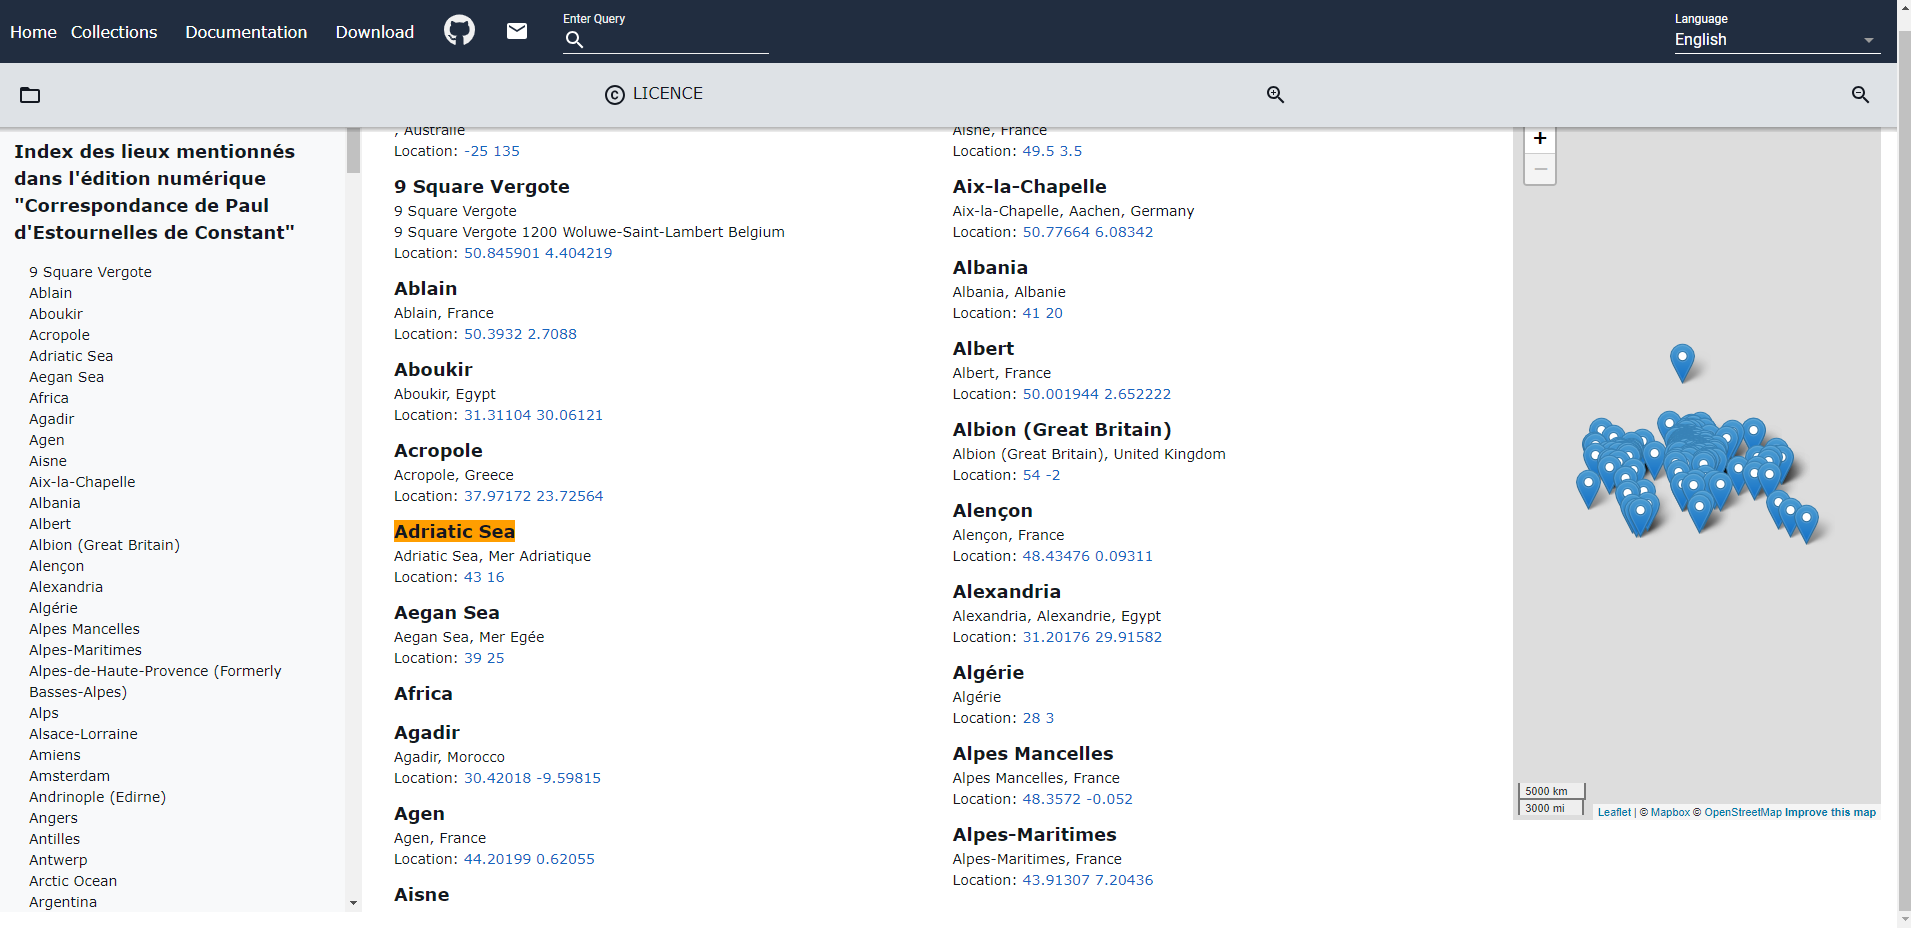
\includegraphics[width=1\linewidth]{schémas/index_places_old.png}
        \caption{Ancien index de DiScholEd}
        \label{fig:schémas18}
    \end{figure}
\begin{figure}[H]
        \centering
        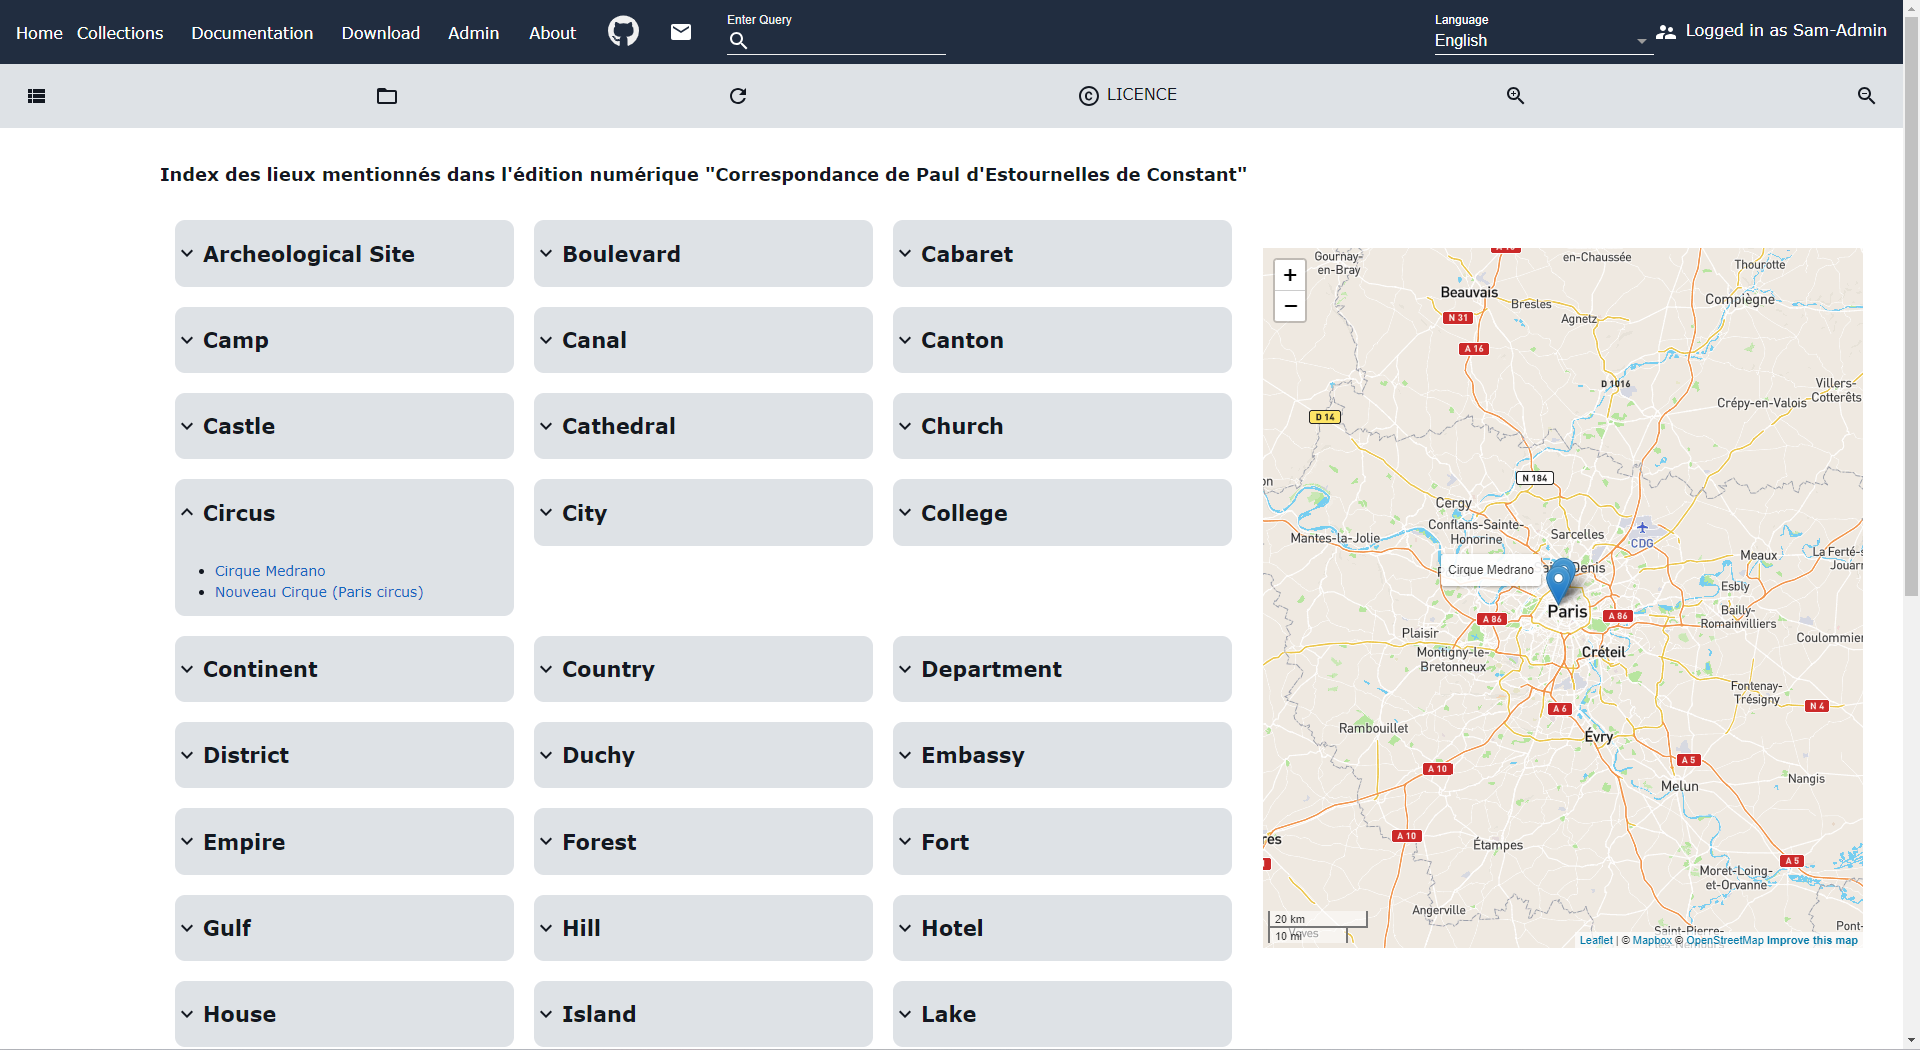
\includegraphics[width=1\linewidth]{schémas/index_places_new.png}
        \caption{Nouvel index de DiScholEd}
        \label{fig:schémas19}
    \end{figure}

\newpage

\section{Modifications des blocs de métadonnées pour toutes les langues}

\begin{figure}[H]
\centering
\begin{minipage}{.5\textwidth}
  \centering
  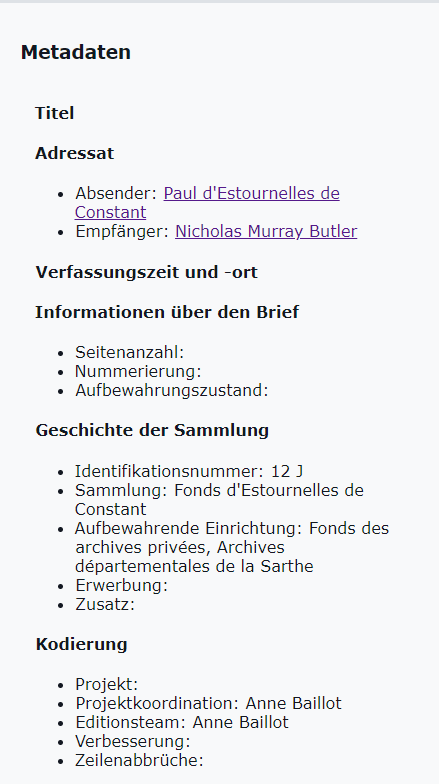
\includegraphics[width=.7\linewidth]{schémas/old_meta_deu.png}
  \caption{Ancien bloc de métadonnées}
  \label{old-meta-deu}
\end{minipage}%
\begin{minipage}{.5\textwidth}
  \centering
  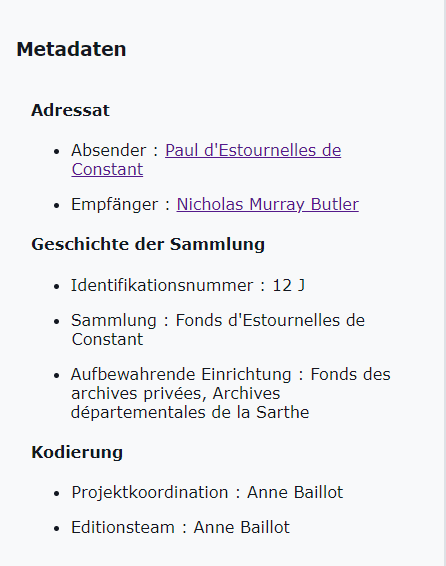
\includegraphics[width=.7\linewidth]{schémas/new-meta-deu.png}
  \caption{Nouveaux blocs de métadonnées sans les entrées où il n'y a pas d'information}
  \label{new-meta-deu}
\end{minipage}
\end{figure}

\newpage

\section{Amélioration de la page de présentation des collections}
\label{old_collection}
\begin{figure}[H]
        \centering
        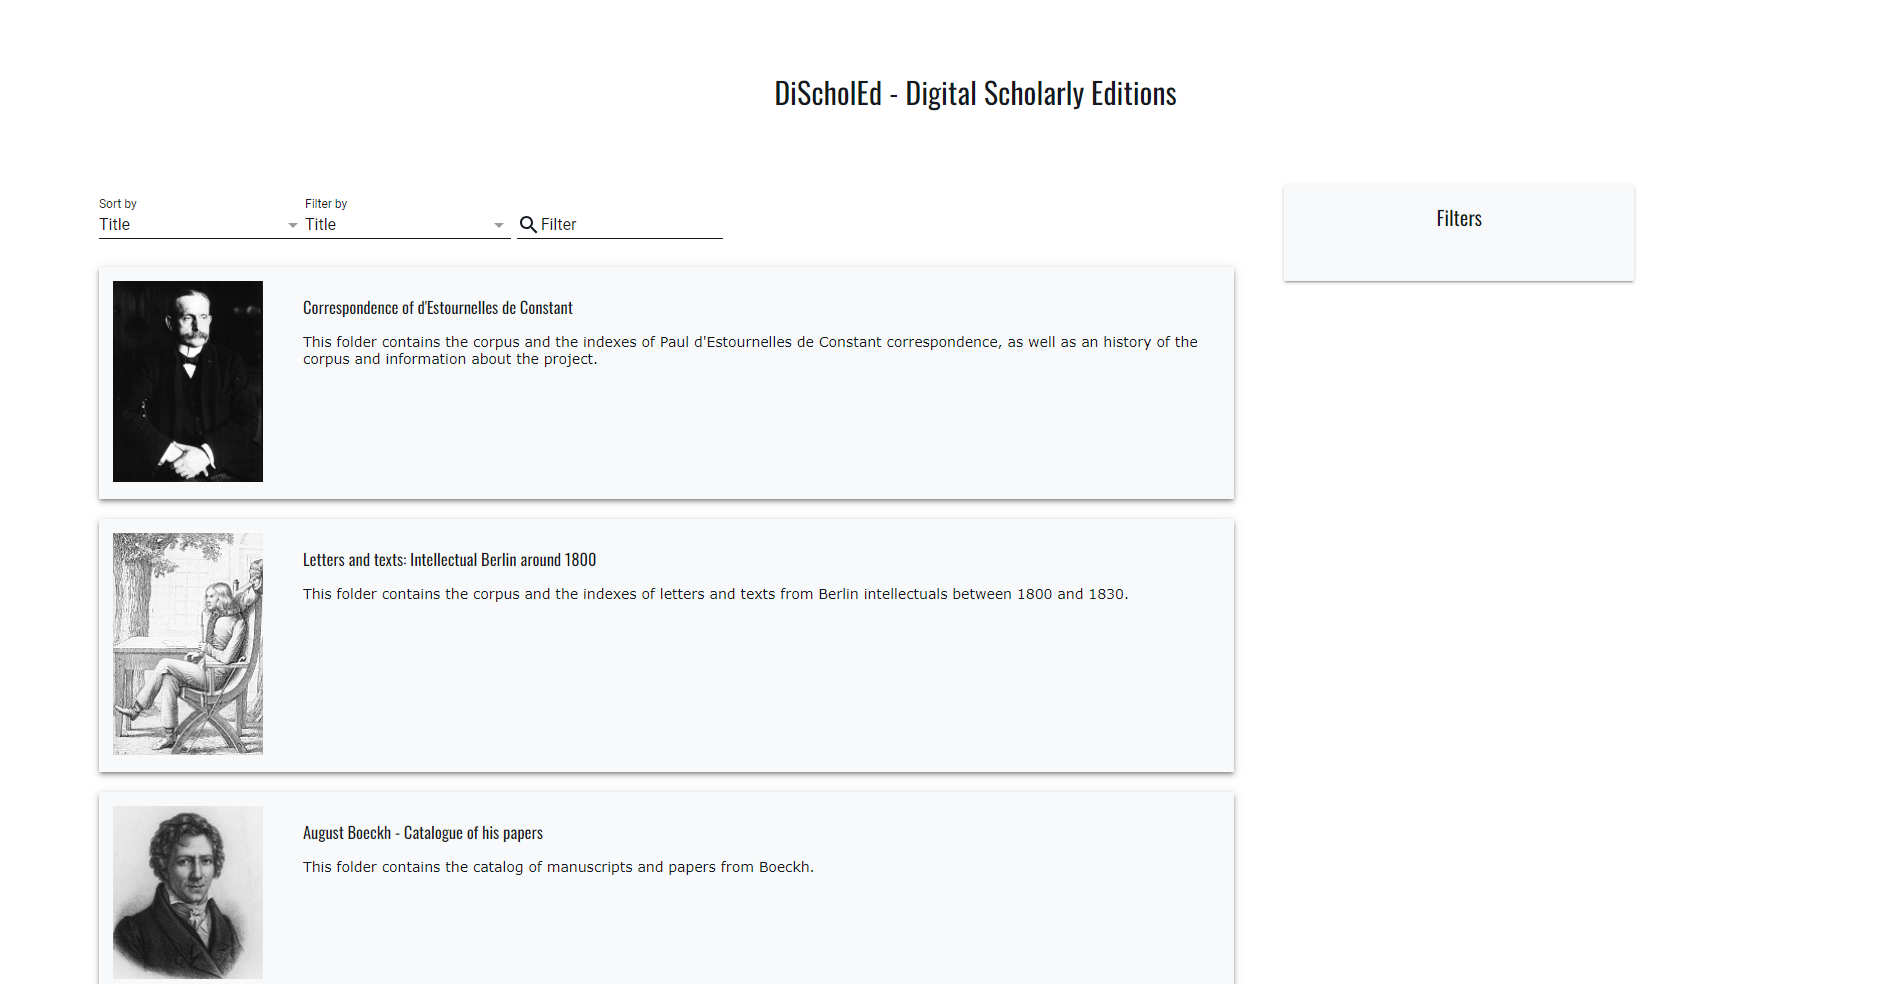
\includegraphics[width=1\linewidth]{schémas/old_collection.png}
        \caption{Ancienne page des collections}
        \label{fig:schémas22}
    \end{figure}
\label{new_collection}
\begin{figure}[H]
        \centering
        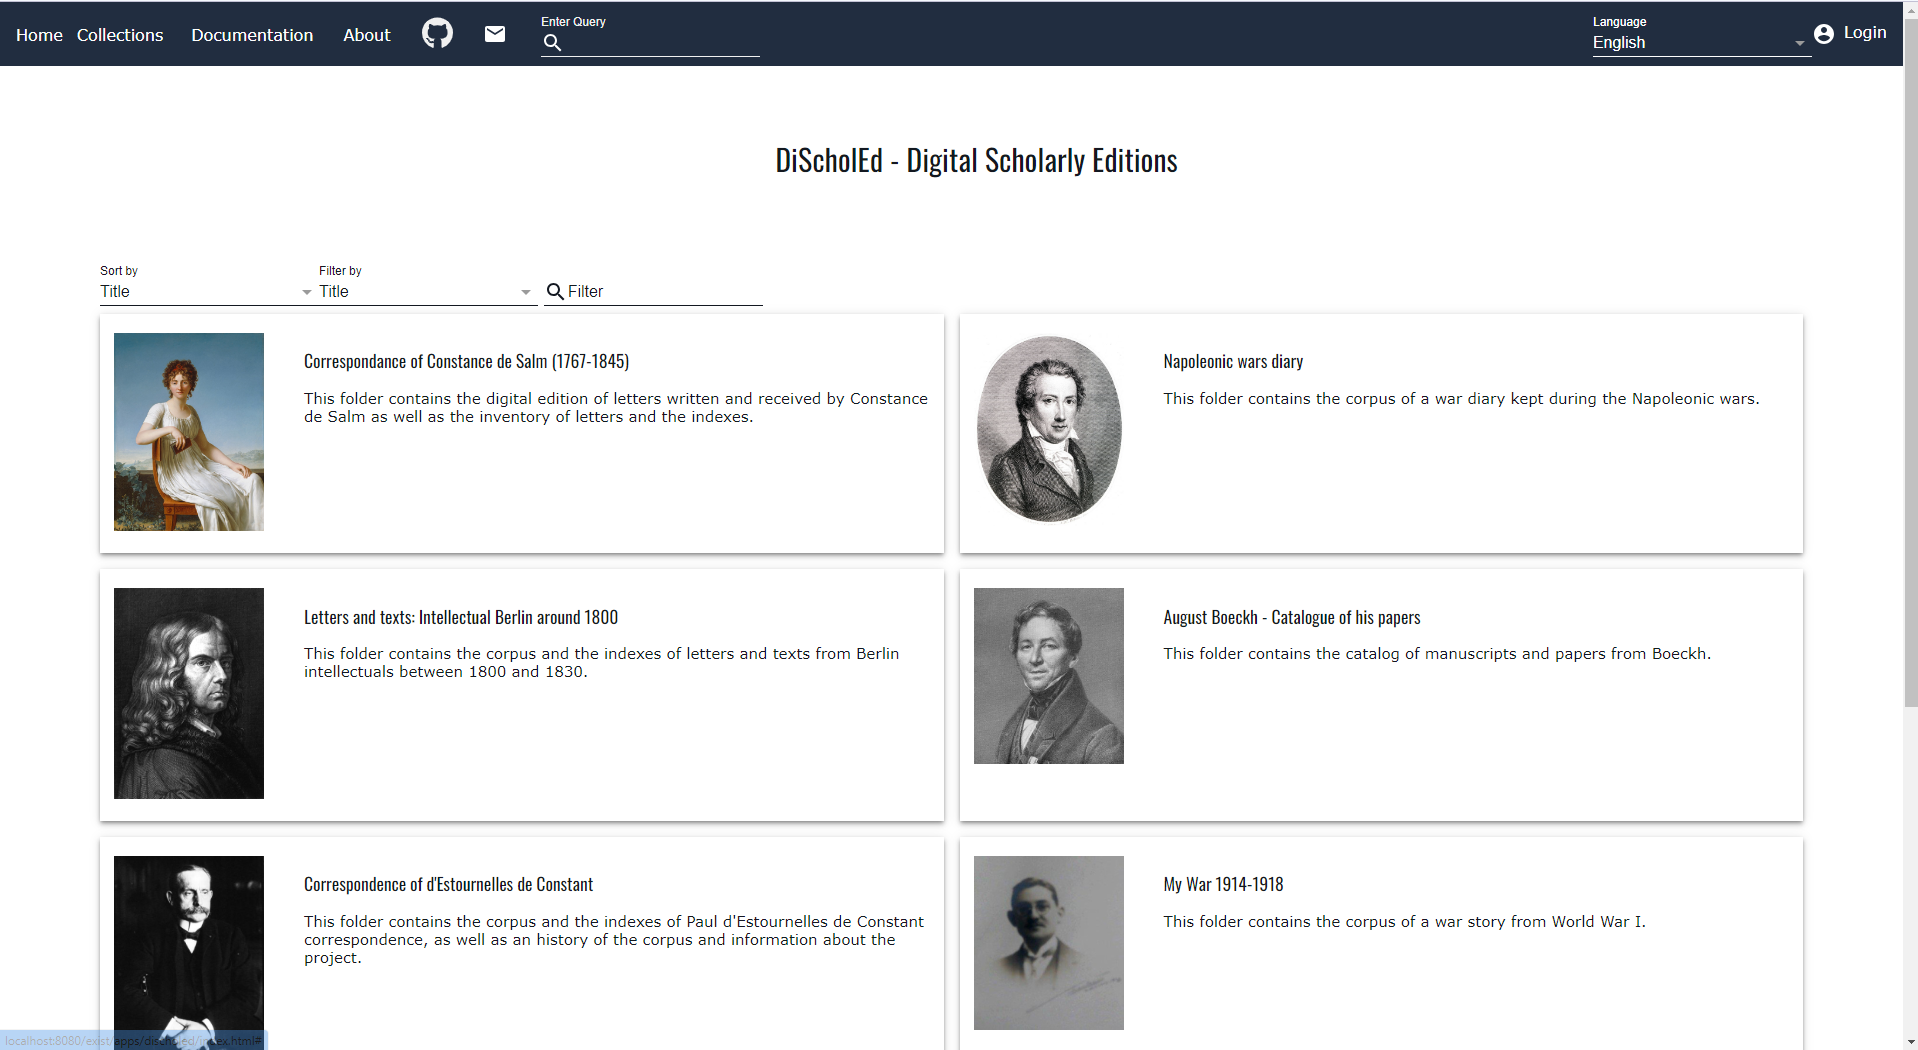
\includegraphics[width=1\linewidth]{schémas/new_collection.png}
        \caption{Nouvelle page des collections (meilleure qualité d'image, blocs cliquables, ordonnée par ordre alphabétique et en colonnes)}
        \label{fig:schémas23}
    \end{figure}

\newpage

\section{Suppression des langues indisponibles}

\begin{figure}[H]
\centering
\begin{minipage}{.5\textwidth}
  \centering
  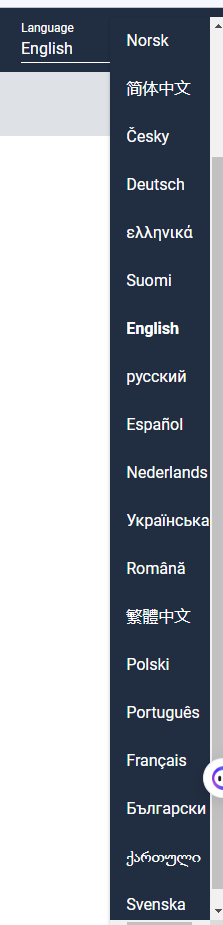
\includegraphics[width=.4\linewidth]{schémas/blangue.png}
  \caption{Anciennes langues non disponibles}
  \label{blangue}
\end{minipage}%
\begin{minipage}{.5\textwidth}
  \centering
  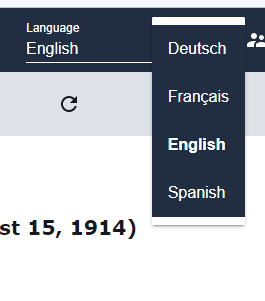
\includegraphics[width=.7\linewidth]{schémas/langue.png}
  \caption{Langues indisponibles de DiScholEd}
  \label{langue}
\end{minipage}
\end{figure}
